\documentclass[a4paper]{article}
\usepackage{cmap}
\usepackage[utf8]{inputenc}
\usepackage[T2A]{fontenc}
\usepackage[english,russian]{babel} 
\usepackage[left=15mm, top=15mm, right=15mm, bottom=30mm, nohead, nofoot]{geometry}
\usepackage{blindtext}  % рыба-текст
\usepackage{graphicx}  % изображения
\usepackage{float} % плавающие объекты
\usepackage{wrapfig}  % изображения
\usepackage{tikz} % графика
\usepackage{mdframed} % рамки
\usepackage{xcolor} % определение цветов
\usepackage{nicefrac} % красивые дроби
\usepackage{cancel} % сокращение
\usepackage{amsmath,amsfonts,amssymb} % математический пакет
\usepackage{hyperref}  % гиперссылки
\usepackage{fancybox,fancyhdr} % хедер и футер
\usepackage{listings} % код
\usepackage[skip=2pt]{caption} % расстояние между подписью и картинкой
\pagestyle{fancy}
\fancyhf{}
\fancyhead[L]{Лабораторная работа №7}
\fancyhead[R]{\textit{Анализ точности систем управления}}
\fancyfoot[C]{\thepage}
\headsep=4mm
\footskip=13mm
\setlength{\parindent}{0em}
\setlength{\parsep}{0em}
\setlength{\headheight}{12pt}
\setlength{\topmargin}{-38pt}
\setlength{\arraycolsep}{2pt}

\definecolor{urlcolor}{HTML}{3454D1}
\definecolor{linkcolor}{HTML}{3454D1}
\hypersetup{
    pdfstartview=FitH,
    linkcolor=linkcolor,
    urlcolor=urlcolor,
    colorlinks=true,
    pdftitle={Лабораторная работа №7},
    pdfauthor={Овчинников П.А.}
}

\definecolor{strings}{rgb}{0,0.6,0}
\definecolor{comments}{rgb}{0,0.3,0}
\definecolor{numbers}{rgb}{0.5,0.5,0.5}
\definecolor{keywords}{rgb}{0.09,0.61,0.95}
\definecolor{background}{rgb}{0.97,0.97,0.97}
\lstdefinestyle{codestyle}{
    backgroundcolor=\color{background},
    commentstyle=\color{comments},
    keywordstyle=\color{keywords},
    stringstyle=\color{strings},
    numberstyle=\tiny\color{numbers},
    basicstyle=\ttfamily\footnotesize,
    breakatwhitespace=false,
    breaklines=true,
    captionpos=b,
    inputencoding=utf8,
    keepspaces=true,
    numbers=left,
    numbersep=5pt,
    showspaces=false,
    showstringspaces=false,
    showtabs=false,
    tabsize=2,
    extendedchars=true,
    literate=
    {а}{{\cyra}}1
    {б}{{\cyrb}}1
    {в}{{\cyrv}}1
    {г}{{\cyrg}}1
    {д}{{\cyrd}}1
    {е}{{\cyre}}1
    {ж}{{\cyrzh}}1
    {з}{{\cyrz}}1
    {и}{{\cyri}}1
    {й}{{\cyrishrt}}1
    {к}{{\cyrk}}1
    {л}{{\cyrl}}1
    {м}{{\cyrm}}1
    {н}{{\cyrn}}1
    {о}{{\cyro}}1
    {п}{{\cyrp}}1
    {р}{{\cyrr}}1
    {с}{{\cyrs}}1
    {т}{{\cyrt}}1
    {у}{{\cyru}}1
    {ф}{{\cyrf}}1
    {х}{{\cyrh}}1
    {ц}{{\cyrc}}1
    {ч}{{\cyrch}}1
    {ш}{{\cyrsh}}1
    {щ}{{\cyrshch}}1
    {ъ}{{\cyrhrdsn}}1
    {ы}{{\cyrery}}1
    {ь}{{\cyrsftsn}}1
    {э}{{\cyrerev}}1
    {ю}{{\cyryu}}1
    {я}{{\cyrya}}1
    {А}{{\CYRA}}1
    {Б}{{\CYRB}}1
    {В}{{\CYRV}}1
    {Г}{{\CYRG}}1
    {Д}{{\CYR96}}1
    {Е}{{\CYRE}}1
    {Ж}{{\CYRZH}}1
    {З}{{\CYRZ}}1
    {И}{{\CYRI}}1
    {Й}{{\CYRISHRT}}1
    {К}{{\CYRK}}1
    {Л}{{\CYRL}}1
    {М}{{\CYRM}}1
    {Н}{{\CYRN}}1
    {О}{{\CYRO}}1
    {П}{{\CYRP}}1
    {Р}{{\CYRR}}1
    {С}{{\CYRS}}1
    {Т}{{\CYRT}}1
    {У}{{\CYRU}}1
    {Ф}{{\CYRF}}1
    {Х}{{\CYRH}}1
    {Ц}{{\CYRC}}1
    {Ч}{{\CYRCH}}1
    {Ш}{{\CYRSH}}1
    {Щ}{{\CYRSHCH}}1
    {Ъ}{{\CYRHRDSN}}1
    {Ы}{{\CYRERY}}1
    {Ь}{{\CYRSFTSN}}1
    {Э}{{\CYREREV}}1
    {Ю}{{\CYRYU}}1
    {Я}{{\CYRYA}}1
}
\lstset{style=codestyle}

\addto\captionsrussian{
  \renewcommand{\contentsname}
    {\centering Содержание}
}
\newcommand{\addsection}[1]{
    \phantomsection
    \addcontentsline{toc}{section}{#1}
    \section*{\centering #1}
}
\newcommand{\addsubsection}[1]{
    \phantomsection
    \addcontentsline{toc}{subsection}{#1}
    \subsection*{\centering #1}
}
\newcommand{\addsubsubsection}[1]{
    \phantomsection
    \addcontentsline{toc}{subsubsection}{#1}
    \subsubsection*{\centering #1}
}

\newmdenv[
    leftmargin = 0.5em,
    skipabove = 0.5em,
    skipbelow = 0.5em,
    linewidth = 1pt,
    rightline = false,
    topline = false,
    bottomline = false
]{quotebox}

\newlength{\tempheight}
\newcommand{\Let}{
\mathbin{\text{\settoheight{\tempheight}{\mathstrut}\raisebox{0.4\pgflinewidth}{
\tikz[baseline=0.5ex,line cap=round,line join=round] \draw (0,0) --++ (0.3em,0) --++ (0,2.3ex) --++ (-0.3em,0);
}}}}
\newcommand*\squared[1]{\tikz[baseline=(char.base)]{
            \node[shape=rectangle,draw,inner sep=4pt] (char) {#1};}}
\newcommand*\msquared[1]{\tikz[baseline=(char.base)]{
            \node[shape=rectangle,draw,inner sep=4pt] (char) {$\displaystyle #1$};}}
\newcommand\argmax[1]{\underset{#1}{\text{argmax}}}
\renewcommand\max[1]{\underset{#1}{\text{max}}}
\newcommand{\at}{\biggr\rvert}
\newcommand{\shiftright}[3]{\makebox[#2][r]{\makebox[#1][l]{#3}}}
\newcommand{\e}{\;\text{e}}
\let\oldint\int
\def\int{\oldint\limits}
\DeclareRobustCommand{\divby}{%
  \mathrel{\vbox{\baselineskip.65ex\lineskiplimit0pt\hbox{.}\hbox{.}\hbox{.}}}%
}

\newcommand\NB{\textbf{N\kern-0.32em\textcolor{red}{B}}}

\begin{document}
\begin{titlepage}
    \begin{center}
    \includegraphics[width=0.18\textwidth]{~/Изображения/itmo_logo.png}\\[10pt]
        Федеральное государственное автономное образовательное \\ учреждение высшего образования \\[6pt]
        САНКТ-ПЕТЕРБУРГСКИЙ НАЦИОНАЛЬНЫЙ \\ ИССЛЕДОВАТЕЛЬСКИЙ УНИВЕРСИТЕТ ИТМО \\[16pt]
        Факультет систем управления и робототехники \vfill
        {\large Лабораторная работа №7} \\[0.5em]
        {\large \textbf{\MakeUppercase{Анализ точности систем управления}}}\\[0.5em]
        Вариант №12
    \end{center}\vfill
    \begin{flushright}
        Студент: Овчинников П.А.\\
        Поток: ЛСАУ R22 бак 4.1.1 \\[0.5em]
        Преподаватели: Лопарев А.В.\\Золотаревич В.П. 
    \end{flushright}\vfill
    \begin{center}
        {\small Санкт-Петербург \\ 2024}
    \end{center}
\end{titlepage}
\setcounter{page}{2}
\tableofcontents\newpage
\textbf{Цель работы:} исследование точностных свойств систем управления.

\addsection{Исследование системы с астатизмом нулевого порядка}
\addsubsection{Условия}
\begin{itemize}
    \item Задана структура системы на рис. \ref{system1};
    \begin{figure}[H]
        \centering
        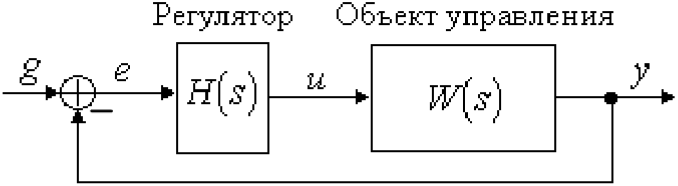
\includegraphics[width=0.5\textwidth]{sources/system1.png}
        \caption{Структурная схема моделируемой системы}
        \label{system1}
    \end{figure}
    \item Передаточная функция объекта управления в соответствии с вариантом:
    $$W(s) = \frac{1}{0.1s^2+0.7s+1};$$
    \item Передаточная функция регулятора: $H(s) = k$;
    \item $k = \{1, 5, 10\}$.
\end{itemize}
\addsubsection{Исследование стационарного режима работы}
\addsubsubsection{Задание}
\begin{itemize}
    \item Задающее воздействие --- $g(t) = A = 4$;
    \item Получить переходные процессы для трёх различных значений $k$;
    \item Определить предельное значение установившейся ошибки $\varepsilon$.
\end{itemize}
% MARK: 1.1
\addsubsubsection{Выполнение работы}
Начнём с того, что составим схему моделирования процесса. Продемонстрирую схему сразу и для стационарного режима работы, и для режима движения с постоянной скоростью:
\begin{figure}[H]
    \centering
    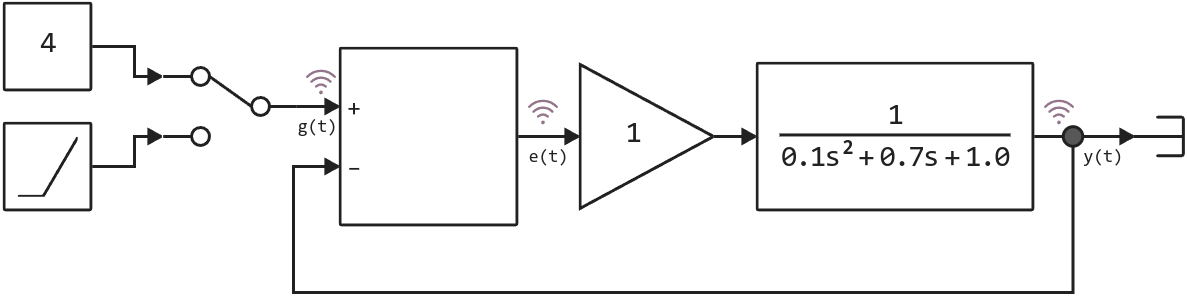
\includegraphics[width=0.66\textwidth]{sources/task1_model.png}
    \caption{Схема моделирования процесса}
    \label{task1_model}
\end{figure}
Т.к. $H(s) = k$, то в качестве регулятора мы можем использовать блок \texttt{Gain}. Задающее воздействие в схеме можно переключать. Схема находится в файле \href{run:sources}{\texttt{task1.engee}}, приложенном к отчёту. Симуляция проведена в среде моделирования и симуляции \href{https://start.engee.com/}{Engee}.\\[0.5em]
Рассчитаем предельное значение установившейся ошибки:
$$\varepsilon = \lim_{s \to 0} \frac{\cancel{s}}{1 + W(s)}\frac{A}{\cancel{s}} = \frac{A}{1+k}$$
Для каждого из значение $k$ при $A = 4$ получаем:
\begin{eqnarray*}
    k = 1: & &\varepsilon = \dfrac{4}{1 + 1} = 2 \\
    k = 5: & &\varepsilon = \dfrac{4}{1 + 5} = \dfrac{2}{3} \\
    k = 10: & &\varepsilon = \dfrac{4}{1 + 10} = \dfrac{4}{11}
\end{eqnarray*}
Построим графики переходных процессов для каждого значения $k$:
\begin{figure}[H]
    \centering
    \begin{minipage}{0.32\textwidth}
        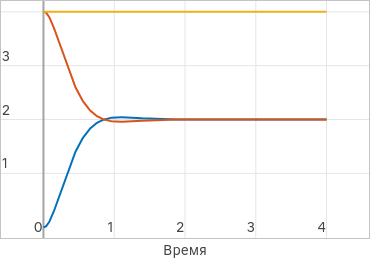
\includegraphics[width=\textwidth]{sources/task1_A_k=1.png}
        \caption*{График процессов для $k = 1$}
    \end{minipage}
    \hfill
    \begin{minipage}{0.32\textwidth}
        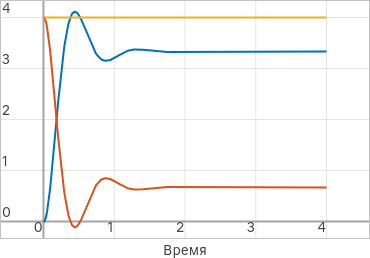
\includegraphics[width=\textwidth]{sources/task1_A_k=5.png}
        \caption*{График процессов для $k = 5$}
    \end{minipage}
    \hfill
    \begin{minipage}{0.32\textwidth}
        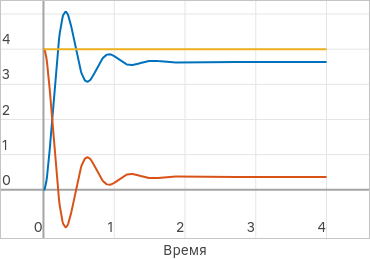
\includegraphics[width=\textwidth]{sources/task1_A_k=10.png}
        \caption*{График процессов для $k = 10$}
    \end{minipage}
\end{figure}
На графиках жёлтый --- $g(t)$, синий --- $y(t)$, красный --- $e(t)$.
\addsubsection{Исследование режима движения с постоянной скоростью}
\addsubsubsection{Задание}
\begin{itemize}
    \item Задающее воздействие --- $g(t) = Vt = 2t$
    \item Получить переходные процессы для трёх различных значений $k$.
\end{itemize}
% MARK: 1.2
\addsubsubsection{Выполнение работы}
Для режима движения с постоянной скоростью схема моделирования, как и говорилось выше, идентична схеме для стационарного режима работы --- она представлена на рис. \ref{task1_model}. Построим графики переходных процессов:
\begin{figure}[H]
    \centering
    \begin{minipage}{0.32\textwidth}
        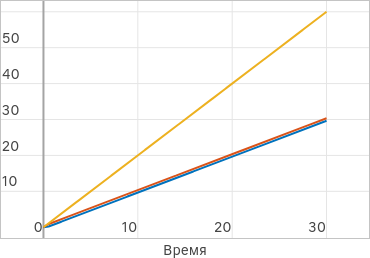
\includegraphics[width=\textwidth]{sources/task1_Vt_k=1.png}
        \caption*{График процессов для $k = 1$}
    \end{minipage}
    \hfill
    \begin{minipage}{0.32\textwidth}
        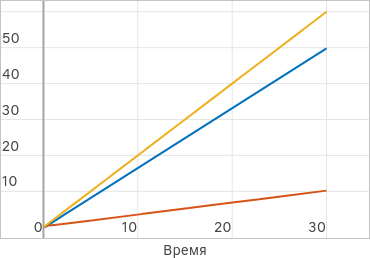
\includegraphics[width=\textwidth]{sources/task1_Vt_k=5.png}
        \caption*{График процессов для $k = 5$}
    \end{minipage}
    \hfill
    \begin{minipage}{0.32\textwidth}
        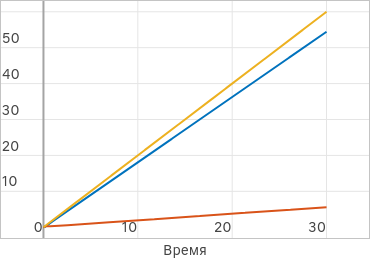
\includegraphics[width=\textwidth]{sources/task1_Vt_k=10.png}
        \caption*{График процессов для $k = 10$}
    \end{minipage}
\end{figure}

\newpage
\addsection{Исследование системы с астатизмом первого порядка}
\addsubsection{Условия}
\begin{itemize}
    \item Задана структура системы на рис. \ref{system1};
    \item Передаточная функция объекта управления в соответствии с вариантом:
    $$W(s) = \frac{s + 1}{0.1s^2+0.7s+1};$$
    \item Передаточная функция регулятора: $H(s) = k/s$;
    \item $k = \{1, 5, 10\}$.
\end{itemize}
\addsubsection{Исследование стационарного режима работы}
\addsubsubsection{Задание}
\begin{itemize}
    \item Задающее воздействие --- $g(t) = A = 4$;
    \item Получить переходные процессы для трёх различных значений $k$;
    \item Определить предельное значение установившейся ошибки $\varepsilon$.
\end{itemize}
% MARK: 2.1
\addsubsubsection{Выполнение работы}
Составим схему моделирования процесса. Продемонстрирую схему сразу для всех режимов работы:
\begin{figure}[H]
    \centering
    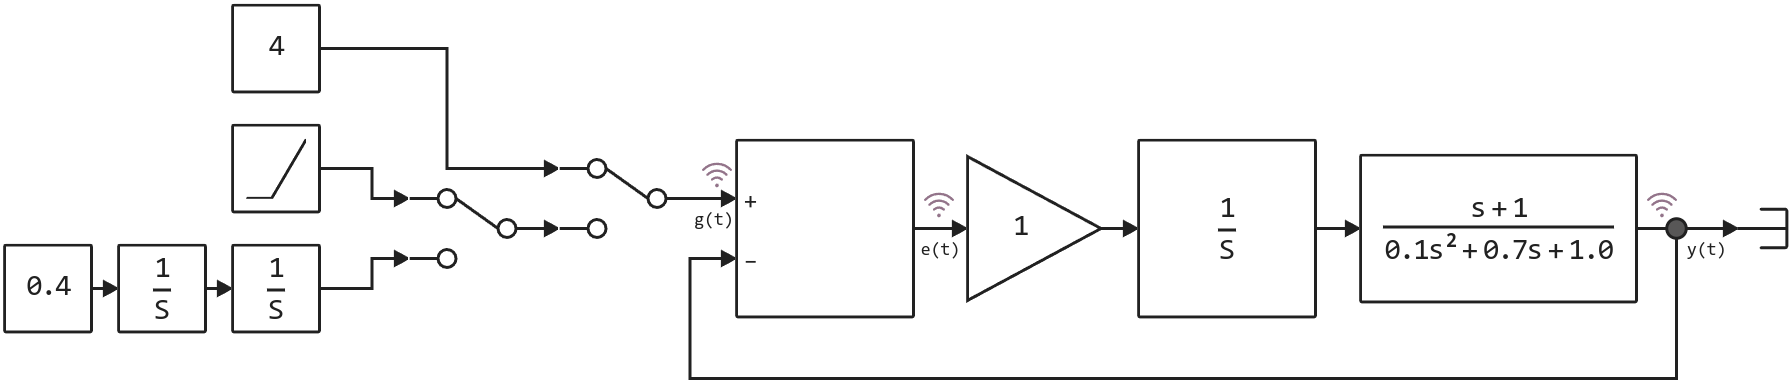
\includegraphics[width=0.8\textwidth]{sources/task2_model.png}
    \caption{Схема моделирования процесса}
    \label{task2_model}
\end{figure}
Регулировать входное воздействие можно через переключатели. Схема находится в файле \href{run:sources}{\texttt{task2.engee}}, приложенном к отчёту. Симуляция проведена в среде моделирования и симуляции \href{https://start.engee.com/}{Engee}.\\[0.5em]
Рассчитаем предельное значение установившейся ошибки для стационарного режима работы с первым порядком астатизма:
$$\varepsilon = \lim_{s \to 0} \frac{\cancel{s}}{1 + W(s)}\frac{A}{\cancel{s}} = \lim_{s\to 0}\frac{A}{1+\frac{W^*(s)}{s}} = \lim_{s \to 0} \frac{As}{s + k} = 0$$
Для любых $k$ и $A$ получаем $\varepsilon = 0$. Построим графики переходных процессов для каждого значения $k$, чтобы убедиться в этом:
\begin{figure}[H]
    \centering
    \begin{minipage}{0.32\textwidth}
        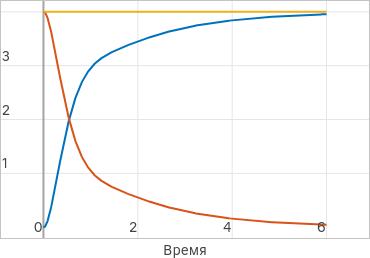
\includegraphics[width=\textwidth]{sources/task2_A_k=1.png}
        \caption*{График процессов для $k = 1$}
    \end{minipage}
    \hfill
    \begin{minipage}{0.32\textwidth}
        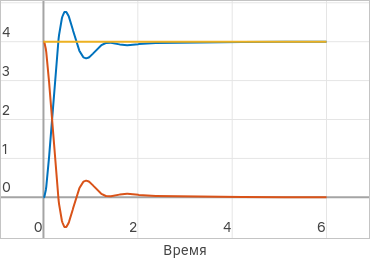
\includegraphics[width=\textwidth]{sources/task2_A_k=5.png}
        \caption*{График процессов для $k = 5$}
    \end{minipage}
    \hfill
    \begin{minipage}{0.32\textwidth}
        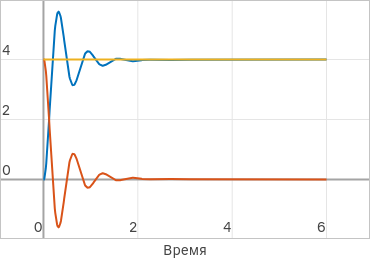
\includegraphics[width=\textwidth]{sources/task2_A_k=10.png}
        \caption*{График процессов для $k = 10$}
    \end{minipage}
\end{figure}
На графиках жёлтый --- $g(t)$, синий --- $y(t)$, красный --- $e(t)$.

\newpage
\addsubsection{Исследование режима движения с постоянной скоростью}
\addsubsubsection{Задание}
\begin{itemize}
    \item Задающее воздействие --- $g(t) = Vt = 2t$
    \item Получить переходные процессы для трёх различных значений $k$;
    \item Определить предельное значение установившейся ошибки $\varepsilon$.
\end{itemize}
% MARK: 2.2
\addsubsubsection{Выполнение работы}
Теперь рассмотрим режим работы с постоянной скоростью. Схема моделирования процесса представлена выше на рис. \ref{task2_model}. Для начала рассчитаем предельное значение установившейся ошибки:
$$\varepsilon = \lim_{s \to 0} \frac{s}{1 + W(s)}\frac{V}{s^2} = \lim_{s \to 0} \frac{\cancel{s}}{s + k}\frac{V}{\cancel{s}} = \frac{V}{k}$$
Для каждого из значение $k$ при $V = 2$ получаем:
$$k = 1: \varepsilon = \dfrac{2}{1} = 2\qquad k = 5: \varepsilon = \dfrac{2}{5} = 0.4 \qquad k = 10: \varepsilon = \dfrac{2}{10} = 0.2$$
Построим графики переходных процессов для каждого значения $k$ с интервалом наблюдения в 30 секунд:
\begin{figure}[H]
    \centering
    \begin{minipage}{0.32\textwidth}
        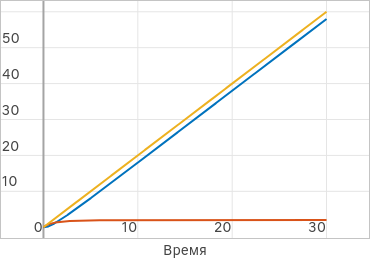
\includegraphics[width=\textwidth]{sources/task2_Vt_k=1.png}
        \caption*{График процессов для $k = 1$}
    \end{minipage}
    \hfill
    \begin{minipage}{0.32\textwidth}
        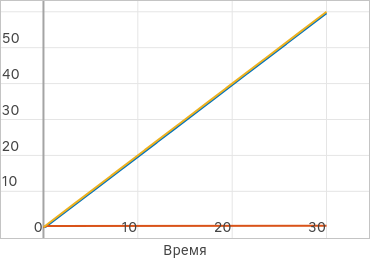
\includegraphics[width=\textwidth]{sources/task2_Vt_k=5.png}
        \caption*{График процессов для $k = 5$}
    \end{minipage}
    \hfill
    \begin{minipage}{0.32\textwidth}
        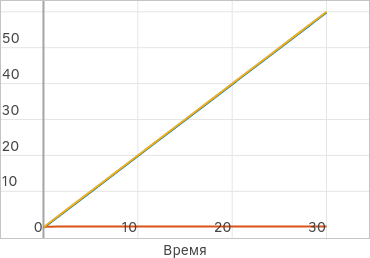
\includegraphics[width=\textwidth]{sources/task2_Vt_k=10.png}
        \caption*{График процессов для $k = 10$}
    \end{minipage}
\end{figure}

\addsubsection{Исследование режима движения с постоянным ускорением}
\addsubsubsection{Задание}
\begin{itemize}
    \item Задающее воздействие --- $g(t) = at^2/2 = 0.4t^2$
    \item Получить переходные процессы для трёх различных значений $k$.
\end{itemize}
% MARK: 2.3
\addsubsubsection{Выполнение работы}
Наконец, перейдём к режиму движения с постоянным ускорением. Схема моделирования процесса, как и всегда, представлена на рис. \ref{task2_model}.\\[0.5em]
Построим графики переходных процессов для каждого значения $k$ на том же интервале наблюдения в 30 секунд:
\begin{figure}[H]
    \centering
    \begin{minipage}{0.32\textwidth}
        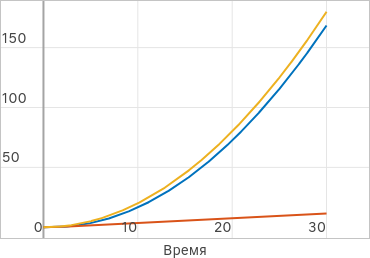
\includegraphics[width=\textwidth]{sources/task2_at2_k=1.png}
        \caption*{График процессов для $k = 1$}
    \end{minipage}
    \hfill
    \begin{minipage}{0.32\textwidth}
        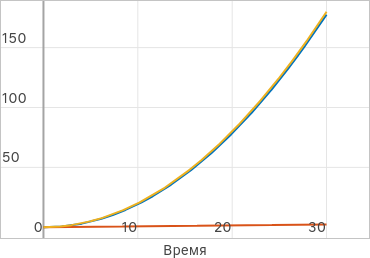
\includegraphics[width=\textwidth]{sources/task2_at2_k=5.png}
        \caption*{График процессов для $k = 5$}
    \end{minipage}
    \hfill
    \begin{minipage}{0.32\textwidth}
        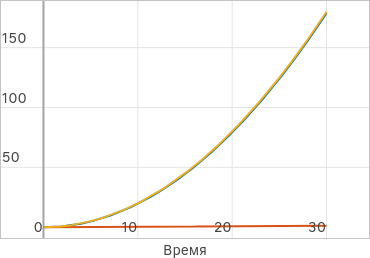
\includegraphics[width=\textwidth]{sources/task2_at2_k=10.png}
        \caption*{График процессов для $k = 10$}
    \end{minipage}
\end{figure}
Как мы видим, при астатизме первого порядка для режима движения с постоянным ускорением установившаяся ошибка стремится к бесконечности, как и в ситуации с постоянной скоростью при отсутствии астатизма.

\addsection{Исследование влияния внешних возмущений}
\addsubsection{Условия и задание}
\begin{itemize}
    \item Функции внешнего возмущения заданы вариантом --- $f_1(t) = 0.5$ и $f_2(t) = -0.4$;
    \item Передаточная функция объекта управления в соответствии с вариантом:
    $$W(s) = \frac{1}{0.1s^2+0.7s+1}.$$
\end{itemize}
\begin{enumerate}
    \item Собрать схему моделирования возмущённой системы по рис. \ref{system2};
    \begin{figure}[H]
        \centering
        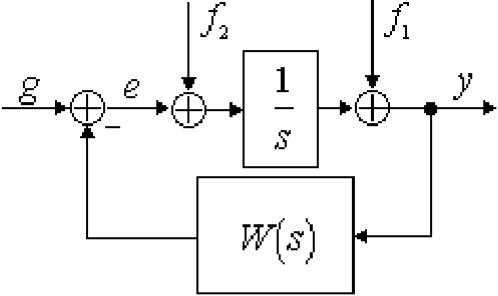
\includegraphics[width=0.4\textwidth]{sources/system2.png}
        \caption{Структурная схема моделируемой системы}
        \label{system2}
    \end{figure}
    \item Полагая $f_2(t) \equiv 0$ и $g(t) = 1(t)$, получить переходный процесс и определить предельное значение установившейся ошибки $\varepsilon$;
    \item Полагая $f_1(t) \equiv 0$ и $g(t) = 1(t)$, получить переходный процесс и определить предельное значение установившейся ошибки $\varepsilon$.
\end{enumerate}
% MARK: 3

\addsubsection{Выполнение работы}
Для начала соберём схему моделирования возмущённой системы. В схеме для моделирования $f_2(t) \equiv 0$ или $f_1(t) \equiv 0$ необходимо занулить соответствующий константный блок. Схема выглядит следующим образом:
\begin{figure}[H]
    \centering
    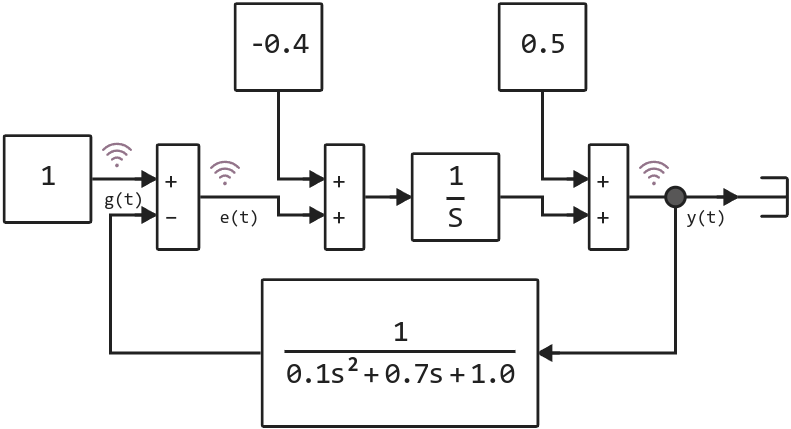
\includegraphics[width=0.56\textwidth]{sources/task3_model.png}
    \caption{Схема моделирования процесса}
    \label{task3_model}
\end{figure}
Смоделировать процесс можно самостоятельно --- схема находится в файле \href{run:sources}{\texttt{task3.engee}}, приложенном к отчёту. Симуляция проведена в среде моделирования и симуляции \href{https://start.engee.com/}{Engee}.\\[0.5em]
Теперь рассчитаем предельное значение установившейся ошибки, воспользовавшись теоретическими сведениями для расчёта ошибки в общем виде:
$$e = g - y = -y = -W(s)\left( f_1 - \frac{f_2 + y}{s} \right) = -W(s)\left( f_1 - \frac{f_2 - e}{s} \right) \quad\Rightarrow\quad \left( 1 + \frac{W(s)}{s} \right)e = \frac{W(s)f_2}{s}-W(s)f_1$$
$$$$
Выражаем $e$:
$$e = \frac{\frac{W(s)}{s}}{1 + \frac{W(s)}{s}}f_2 - \frac{W(s)}{1 + \frac{W(s)}{s}}f_1 = \frac{W(s)}{s + W(s)}f_2 - \frac{sW(s)}{s + W(s)}f_1$$
Теперь рассчитаем предельное значение:
$$\varepsilon = \lim_{s \to 0} \left[ \frac{W(s)}{s + W(s)}f_2 - \frac{sW(s)}{s + W(s)}f_1 \right] = f_2$$
То есть ошибка всегда стремится к значению внешнего возмущения $f_2$.\\[0.5em]
Положим $f_2(t) \equiv 0$ и $g(t) = 1(t)$. Построим график переходного процесса и убедимся в том, что установившаяся ошибка для этого случая стремится к нулю:
\begin{figure}[H]
    \centering
    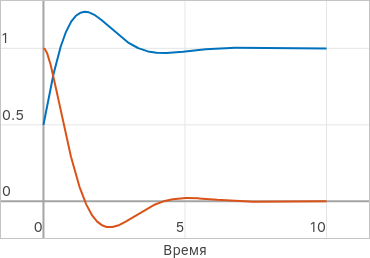
\includegraphics[width=0.32\textwidth]{sources/task3_f2=0.png}
    \caption{График процессов для $f_2(t) \equiv 0$}
\end{figure}
Красным обозначена ошибка $e(t)$, синим --- $y(t)$.\\[0.5em]
Теперь положим $f_1(t) \equiv 0$ и $g(t) = 1(t)$. Построим график переходного процесса и убедимся в том, что установившаяся ошибка для этого случая стремится к значению внешнего возмущения $f_2$:
\begin{figure}[H]
    \centering
    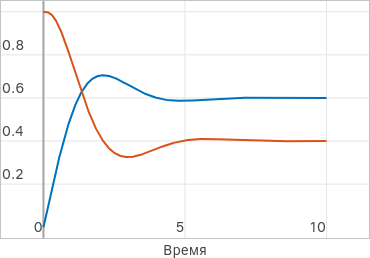
\includegraphics[width=0.4\textwidth]{sources/task3_f1=0.png}
    \caption{График процессов для $f_1(t) \equiv 0$}
\end{figure}
Видим, что красный график, которым обозначена ошибка $e(t)$, как раз стремится к $0.4$.

\addsection{Исследование установившейся ошибки при произвольном входном воздействии}
\addsubsection{Условия и задание}
\begin{itemize}
    \item Структура системы представлена на рис. \ref{system1};
    \item Передаточная функция объекта управления в соответствии с вариантом:
    $$W(s) = \frac{1}{0.1s^2+0.7s+1};$$
    \item Передаточная функция регулятора: $H(s) = 1$;
    \item Входное воздействие --- $g(t) = 2 + \cos{0.5t}$.
\end{itemize}
\begin{enumerate}
    \item Получить переходный процесс в замкнутой системе и определить (по графику) установившуюся ошибку слежения $e_y(t)$;
    \item Получить приближённое аналитическое выражение для $e_y(t)$, сохранив в ряде Тейлора первые три члена;
    \item Построить график $e_y(t)$ в соответствии с полученным аналитическим выражением (использовать для этого блок нелинейных функций Fnc).
\end{enumerate}
% MARK: 4
\addsubsection{Выполнение работы}
Для начала, как и всегда, соберём схему моделирования процесса. Схема представлена на рис. \ref{task4_model}. Т.к. $H(s) = 1$, блок регулятора можно не использовать в схеме, т.к. он будет эквивалентен блоку \texttt{Gain} с параметром 1.
\begin{figure}[H]
    \centering
    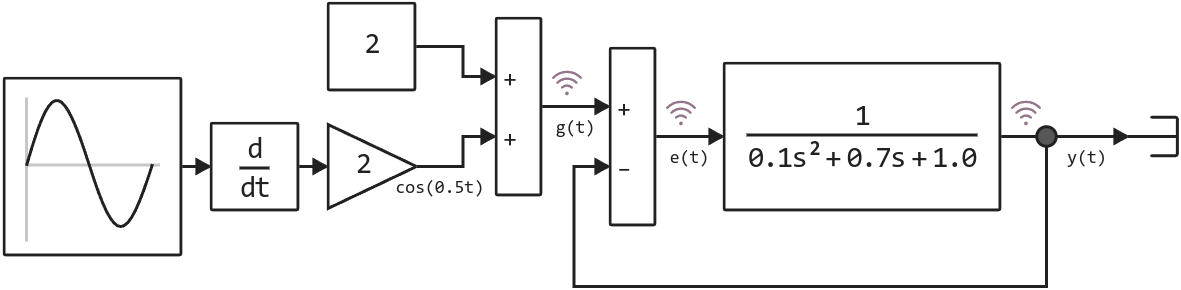
\includegraphics[width=0.7\textwidth]{sources/task4_model.png}
    \caption{Схема моделирования процесса}
    \label{task4_model}
\end{figure}
Схема находится в файле \href{run:sources}{\texttt{task4.engee}}, приложенном к отчёту. Симуляция проведена в среде моделирования и симуляции \href{https://start.engee.com/}{Engee}.\\[0.5em]
Построим график переходного процесса и постараемся определить установившуюся ошибку слежения $e_y(t)$:
\begin{figure}[H]
    \centering
    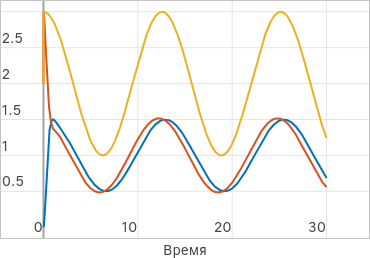
\includegraphics[width=0.4\textwidth]{sources/task4_graphics.png}
    \caption{График процессов для $g(t) = 2 + \cos{0.5t}$}
\end{figure}
Здесь, как и на графиках выше, красным обозначена ошибка $e(t)$, синим --- $y(t)$, а жёлтым --- $g(t)$.\\[0.5em]
Очевидно, учитывая характер входного воздействия, что ошибка в пределе не установится и будет колебаться вокруг некоторого значения.\\[0.5em]
В таком случае попробуем приблизить установившуюся ошибку $e_y(t)$ аналитически. Величина предельного значения установившейся ошибки может быть рассчитана по передаточной функции системы. Образы входного сигнала и ошибки слежения связаны таким соотношением:
$$E(s) = \Phi_e(s)G(s),$$
где $E(s) = \mathcal{L}\{e(t)\}$, $G(s) = \mathcal{L}\{g(t)\}$, а $\Phi_e(s)$ --- передаточная функция замкнутой системы по ошибке слежения относительно задающего воздействия. Последний вычисляется следующим образом:
$$\Phi_e(s) = \frac{1}{1 + W(s)} = \frac{1}{1 + \dfrac{1}{0.1s^2+0.7s+1}} = \frac{0.1s^2 + 0.7s + 1}{0.1s^2 + 0.7s + 2}$$
Для приближённой оценки ошибки слежения разложим $\Phi_e(s)$ в ряд Тейлора в окрестности нуля:
$$\Phi_e(s) = c_0 + c_1s + \frac{c_2}{2!}s^2 + \ldots$$
Принимая во внимание, что $c_i = \left[ d^i\Phi_e(s)/ds^i \right]_{s=0}, i\geqslant 0$ мы получим выражение установившейся ошибки относительно входного воздействия:
$$e_y(t) = c_0g(t) + c_1\dot{g}(t) + \frac{c_2}{2}\ddot{g}(t) + \ldots$$
Для начала вычислим коэффициенты $c_i$:
\begin{eqnarray*}
    c_0 =& \left. \dfrac{0.1s^2 + 0.7s + 1}{0.1s^2 + 0.7s + 2} \right|_{s=0} = \dfrac{1}{2} &= 0.5 \\
    c_1 =& \left. \dfrac{d}{ds}\left( \dfrac{0.1s^2 + 0.7s + 1}{0.1s^2 + 0.7s + 2} \right) \right|_{s=0} = \left.\dfrac{20s+70}{s^4+14s^3+89s^2+280s+700}\right|_{s=0} = \dfrac{70}{700} &= 0.1 \\
    c_2 =& \left. \dfrac{d^2}{ds^2}\left( \dfrac{0.1s^2 + 0.7s + 1}{0.1s^2 + 0.7s + 2} \right) \right|_{s=0} = \left. -\dfrac{60s^{2}+420s+580}{s^{6}+21s^{5}+207s^{4}+1183s^{3}+4140s^{2}+8400s+8000} \right|_{s=0}= \dfrac{580}{8000} &= 0.0725
\end{eqnarray*}
Теперь рассчитаем производные $g(t)$:
\begin{eqnarray*}
    g(t) &=& 2 + \cos{0.5t} \\
    \dot{g}(t) &=& -0.5\sin{0.5t} \\
    \ddot{g}(t) &=& -0.25\cos{0.5t}
\end{eqnarray*}
Итак, соберём всё воедино, чтобы получить разложение для ошибки слежения до третьего члена:
$$e_y(t) = 0.5\left( 2 + \cos{0.5t} \right) + 0.1(-0.5\sin{0.5t}) + \frac{0.0725}{2}(-0.25\cos{0.5t}) = 1 + 0.4909375\cos{0.5t} - 0.05\sin{0.5t}$$
И построим график этой функции в среде моделирования:
\begin{figure}[H]
    \centering
    \begin{minipage}{0.4\textwidth}
        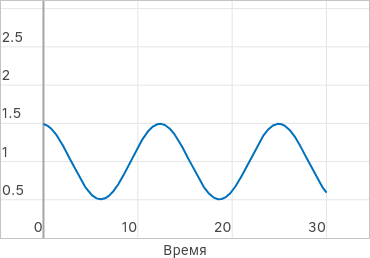
\includegraphics[width=\textwidth]{sources/task4_e_graphics.png}
        \caption*{\centering График $e_y(t)$}
    \end{minipage}
    \hspace{2em}
    \begin{minipage}{0.4\textwidth}
        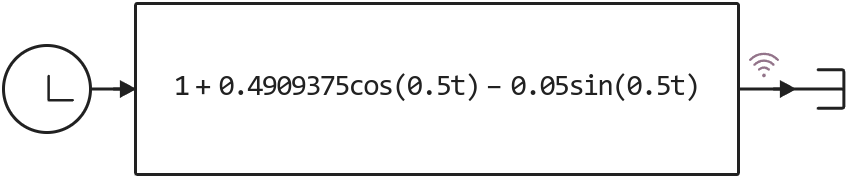
\includegraphics[width=\textwidth]{sources/task4_e_model.png}
        \caption*{\centering Схема моделирования $e_y(t)$}
    \end{minipage}
\end{figure}
На графике видно, что аналитическое выражение для установившейся ошибки слежения $e_y(t)$ \href{https://ru.wikipedia.org/wiki/Сходимость_почти_всюду}{сходится почти всюду} с графиком ошибки, полученным в результате моделирования системы.

\addsection{Выводы}
В ходе выполнения лабораторной работы были исследованы точностные свойства систем управления. Мы рассмотрели системы с астатизмом нулевого и первого порядка, а также системы с внешними возмущениями. Были получены переходные процессы для различных значений коэффициента усиления $k$ регулятора и различных входных воздействий, и мы рассчитали предельные значения установившейся ошибки для каждого случая вручную и сравнили результаты с графиками. Кроме того, было проведено исследование установившейся ошибки при произвольном входном воздействии --- наличие или отсутствие установившейся ошибки следует оценивать для каждого возмущения в системе независимо от порядка астатизма системы. В результате работы были получены навыки работы с системами управления и их анализа, а также понимание влияния различных параметров на точность системы управления.

\end{document}